% ======================================================
%  3 — ARCHITECTURE
% ======================================================
\section{System Architecture}

% --- 3.1 Pipeline overview ---
\begin{frame}{The Pipeline at a Glance}
  \begin{center}
    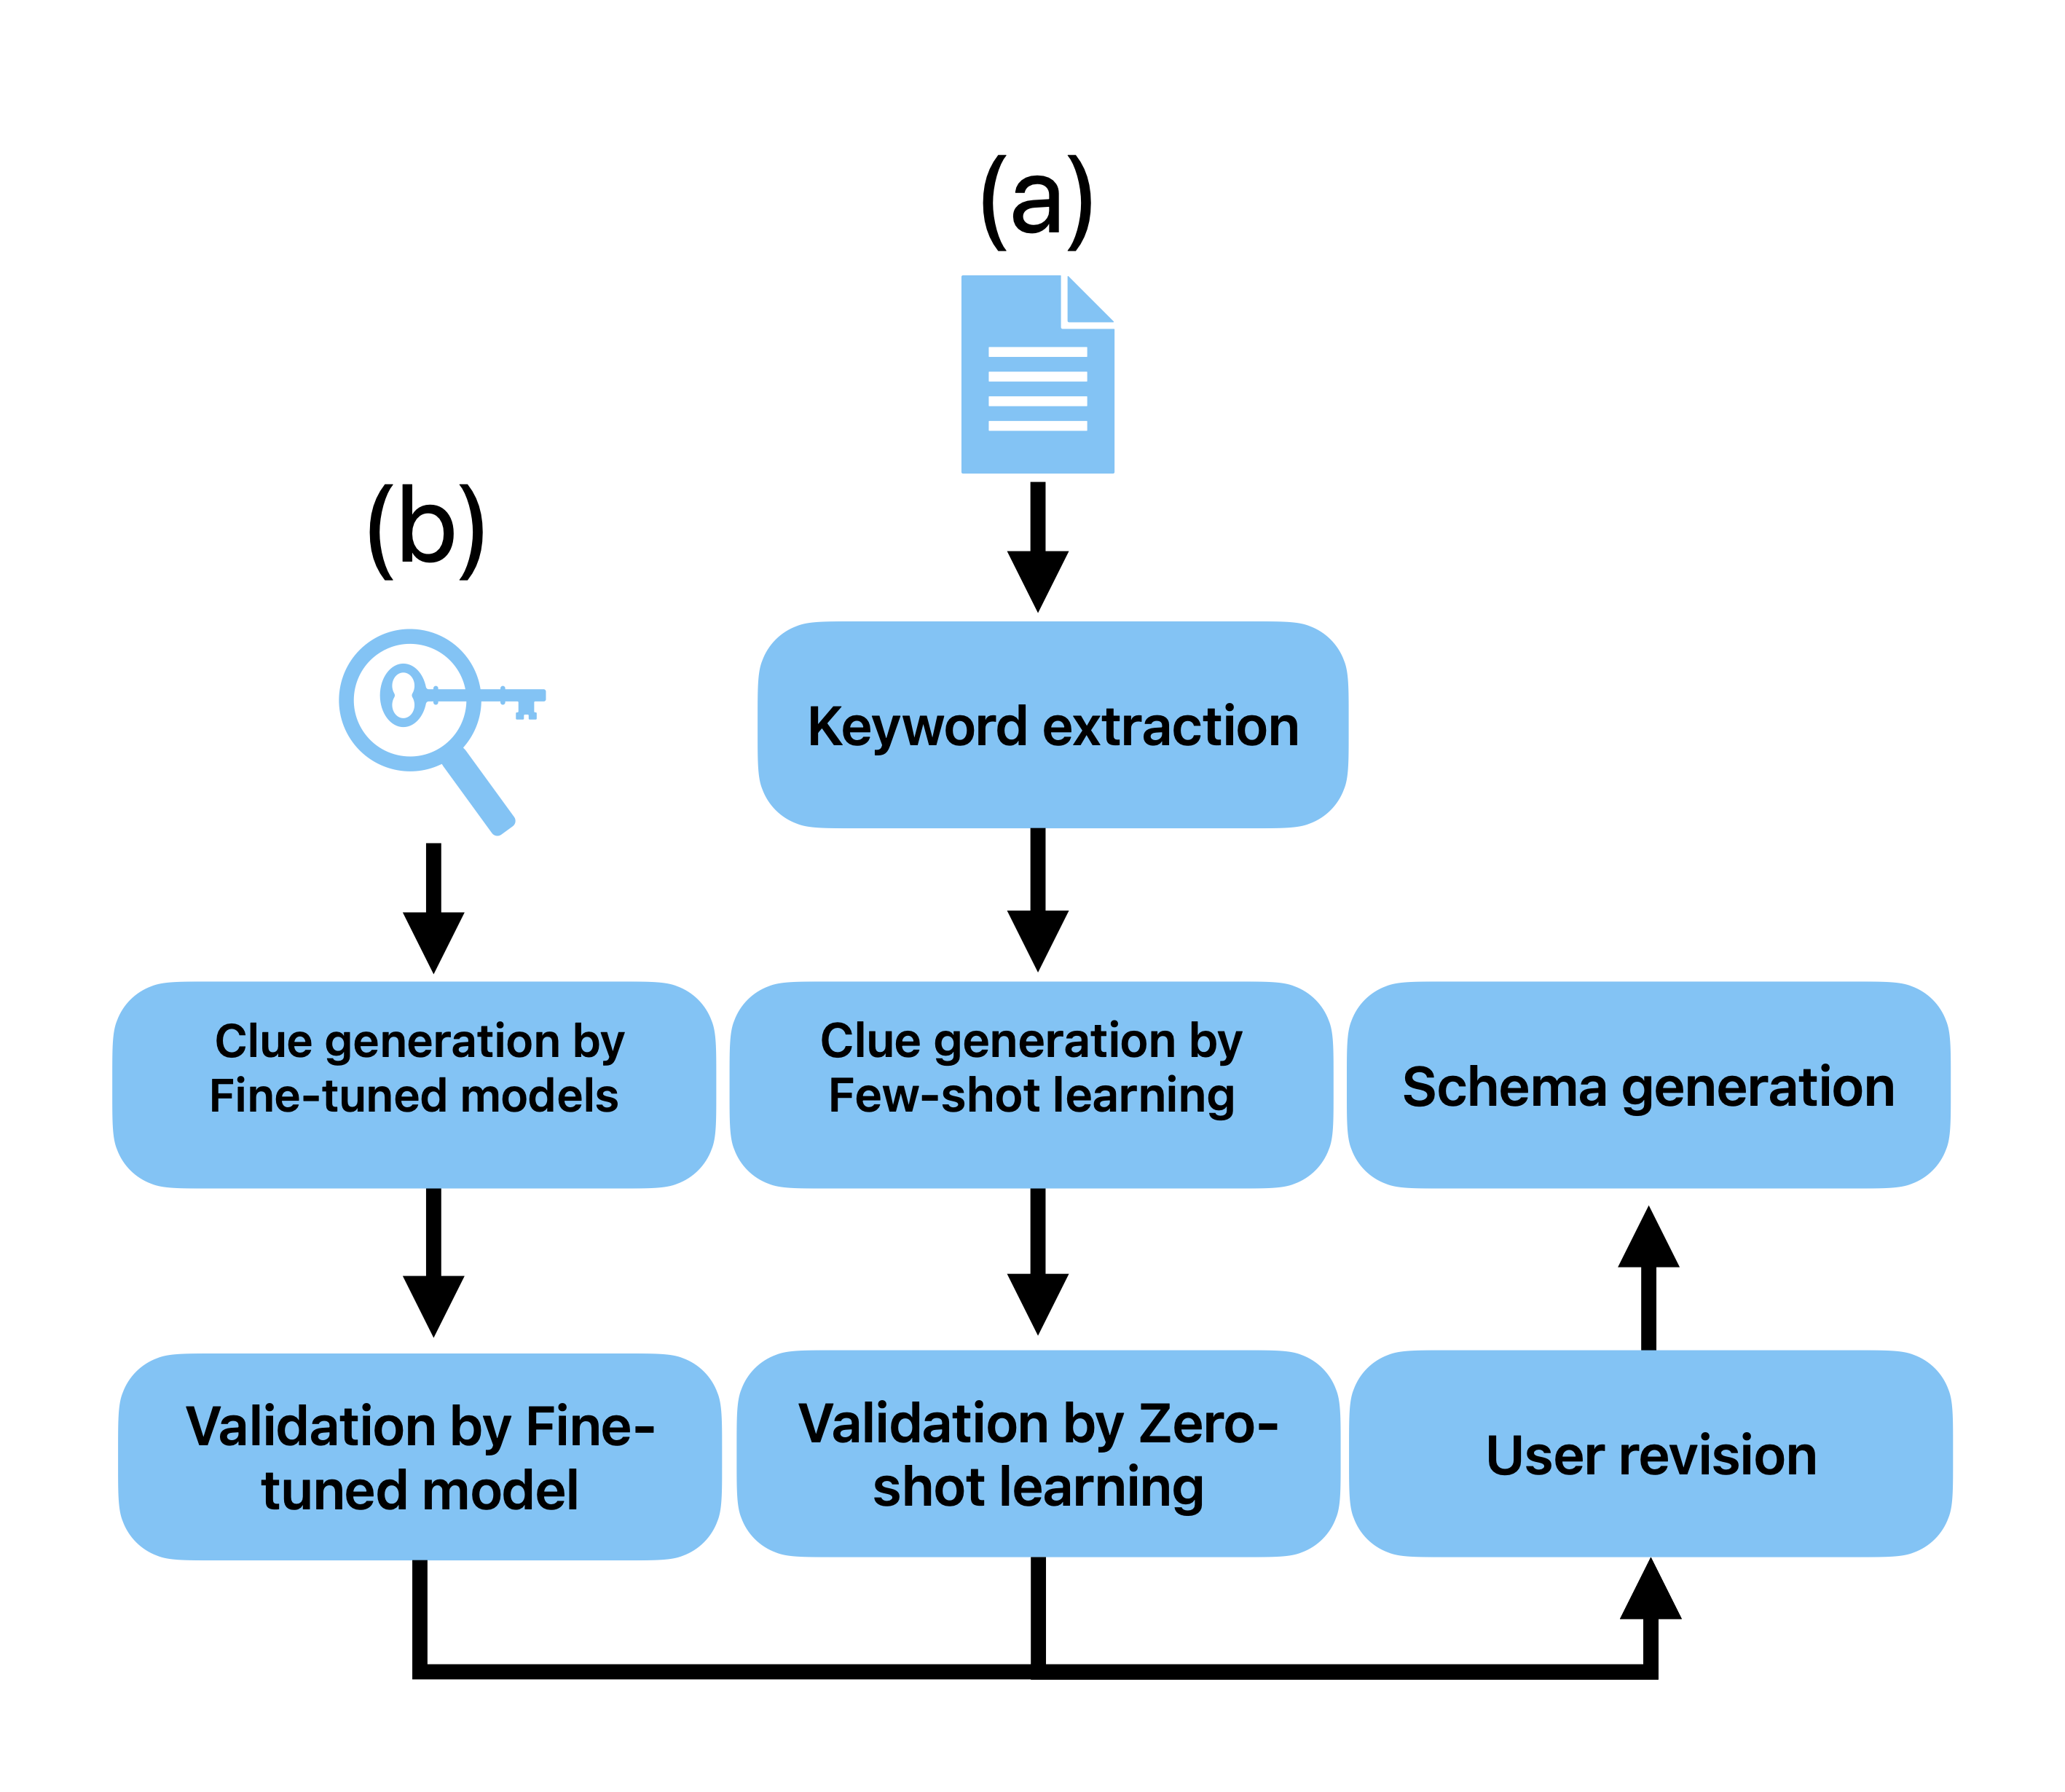
\includegraphics[width=0.82\textwidth]{figures/fig2.png}
  \end{center}
  \vspace{0.5em}
  \begin{columns}[t]
    \column{0.45\textwidth}
      \centering
      {\small\textbf{Path (a)}: Text $\rightarrow$ Keywords $\rightarrow$ Clues}
    \column{0.45\textwidth}
      \centering
      {\small\textbf{Path (b)}: Keywords $\rightarrow$ Clues}
  \end{columns}
  \vspace{0.3em}
  \centering{\small\color{graytext} Both paths converge into validation, human revision, and grid assembly.}
\end{frame}

% --- 3.2 Keyword extraction ---
\begin{frame}{Step 1: Keyword Extraction (from Text)}
  \begin{columns}[c]
    \column{0.55\textwidth}
      \small
      Given any educational text, the LLM extracts\\
      pedagogically relevant keywords\\
      in a \textbf{zero-shot} setting.\\[1em]
      \textbf{Criteria for a good keyword:}
      \vspace{0.3em}
      \begin{itemize}
        \setlength\itemsep{0.4em}
        \item Central to the topic
        \item Suitable as a crossword answer\\
              (single word, appropriate length)
        \item Worth reinforcing for the learner
      \end{itemize}
    \column{0.45\textwidth}
      \centering
      \begin{tikzpicture}[
        box/.style={draw=unisired, rounded corners=6pt, minimum width=4cm, minimum height=1cm, align=center, font=\small, fill=unisired!5, line width=0.7pt},
        arr/.style={->, >=Stealth, line width=1pt, unisired!60}
      ]
      \node[box, fill=unisired!12, font=\small\bfseries] (text) at (0, 3.5) {Input Text};
      \node[box] (llm) at (0, 1.8) {LLM (zero-shot)};
      \node[box, fill=unisired!12, font=\small\bfseries] (kw) at (0, 0) {Keywords};
      \draw[arr] (text) -- (llm);
      \draw[arr] (llm) -- (kw);

      \node[font=\scriptsize, text=graytext, right] at (2.2, 3.5) {\textit{``Photosynthesis}};
      \node[font=\scriptsize, text=graytext, right] at (2.2, 3.0) {\textit{converts light\ldots''}};
      \node[font=\scriptsize, text=unisired, right] at (2.2, 0) {\textbf{chlorophyll}};
      \end{tikzpicture}
  \end{columns}
  \vfill
  \centering
  {\small Result: $\approx$ \textbf{80\%} of extracted keywords rated suitable by evaluators.}
\end{frame}

% --- 3.3 Clue generation ---
\begin{frame}{Step 2: Clue Generation}
  \begin{columns}[c]
    \column{0.5\textwidth}
      \centering
      \begin{tikzpicture}[
        box/.style={draw=unisired, rounded corners=5pt, minimum width=4cm, minimum height=0.8cm, align=center, font=\small, fill=unisired!5, line width=0.7pt},
        arr/.style={->, >=Stealth, line width=1pt, unisired!60}
      ]
      \node[font=\small\bfseries, text=unisired] at (0, 4.2) {From Text (Path A)};
      \node[box] (ctx) at (0, 3.2) {Text + Keywords};
      \node[box] (fs) at (0, 1.8) {Few-shot LLM};
      \node[box, fill=unisired!12] (clue1) at (0, 0.4) {Contextual Clues};
      \draw[arr] (ctx) -- (fs);
      \draw[arr] (fs) -- (clue1);
      \end{tikzpicture}
    \column{0.5\textwidth}
      \centering
      \begin{tikzpicture}[
        box/.style={draw=accentblue, rounded corners=5pt, minimum width=4cm, minimum height=0.8cm, align=center, font=\small, fill=accentblue!5, line width=0.7pt},
        arr/.style={->, >=Stealth, line width=1pt, accentblue!60}
      ]
      \node[font=\small\bfseries, text=accentblue] at (0, 4.2) {From Keywords (Path B)};
      \node[box] (kw) at (0, 3.2) {Keyword List};
      \node[box] (ft) at (0, 1.8) {Fine-tuned LLM};
      \node[box, fill=accentblue!12] (clue2) at (0, 0.4) {Crossword-style Clues};
      \draw[arr] (kw) -- (ft);
      \draw[arr] (ft) -- (clue2);
      \end{tikzpicture}
  \end{columns}
  \vfill
  \centering
  {\small From text: \textbf{70--77\%} acceptable \hspace{2em}
         From keywords: $\approx$ \textbf{60\%} with largest model}
\end{frame}

% --- 3.4 Grid generation ---
\begin{frame}{Step 3: Grid Generation}
  \begin{columns}[c]
    \column{0.55\textwidth}
      \small
      \textbf{Incremental greedy placement} with scoring:
      \vspace{0.4em}
      \begin{enumerate}
        \setlength\itemsep{0.4em}
        \item Start with the longest word
        \item For each remaining word, find\\
              the best intersection with placed words
        \item Score each candidate placement:
      \end{enumerate}
      \vspace{0.3em}
      \begin{equation*}
        S = \alpha \cdot I + \beta \cdot C - \gamma \cdot D
      \end{equation*}
      {\scriptsize\color{graytext} $I$ = intersections \quad $C$ = compactness \quad $D$ = density penalty}
      \vspace{0.4em}
      \begin{enumerate}
        \setcounter{enumi}{3}
        \item Stop when score degrades\\or all words are placed
      \end{enumerate}
    \column{0.45\textwidth}
      \centering
      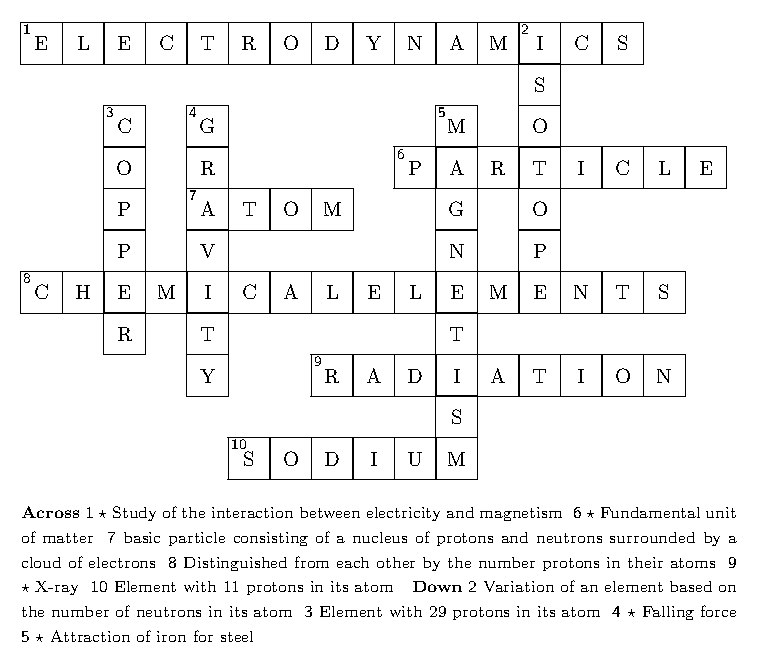
\includegraphics[width=0.78\textwidth]{figures/crossword.pdf}\\[0.5em]
      {\scriptsize\color{graytext} Example of a generated crossword grid}
  \end{columns}
\end{frame}

% --- 3.5 Results summary ---
\begin{frame}{End-to-End Evaluation}
  \vspace{0.5em}
  \begin{columns}[c]
    \column{0.33\textwidth}\centering
      \fcolorbox{unisired}{unisired!5}{\parbox{3cm}{\centering\vspace{0.4em}
      {\LARGE\color{unisired}\textbf{$\sim$80\%}}\\[0.2em]
      {\small Keyword\\Extraction\\Suitability}\vspace{0.4em}}}
    \column{0.33\textwidth}\centering
      \fcolorbox{unisired}{unisired!10}{\parbox{3cm}{\centering\vspace{0.4em}
      {\LARGE\color{unisired}\textbf{70--77\%}}\\[0.2em]
      {\small Acceptable\\Clues\\(from text)}\vspace{0.4em}}}
    \column{0.33\textwidth}\centering
      \fcolorbox{unisired}{unisired!15}{\parbox{3cm}{\centering\vspace{0.4em}
      {\LARGE\color{unisired}\textbf{$\sim$70\%}}\\[0.2em]
      {\small Flawed Clues\\Detected\\Automatically}\vspace{0.4em}}}
  \end{columns}
  \vfill
  \centering
  {\small Human-in-the-loop revision ensures final quality for classroom use.}
\end{frame}